% !TeX spellcheck = en_US
\documentclass[11pt,a4paper,twocolumn]{book}
\usepackage[latin1]{inputenc}
\usepackage{amsmath}
\usepackage{amsfonts}
\usepackage{amssymb}
\usepackage{graphicx}
\usepackage[table]{xcolor}
\usepackage{wrapfig}
\usepackage{multicol}
\usepackage{multirow}
\usepackage{paralist}
\usepackage{longtable}
\usepackage{tabu}
\usepackage{soul}
\usepackage{titling}
\usepackage{pdfpages}
\usepackage[hidelinks]{hyperref}

\hypersetup{
	colorlinks,
	citecolor=black,
	filecolor=black,
	linkcolor=black,
	urlcolor=black
}

\title{Fallout Equestria: Wasteland Ventures}
\date{\today} 


\begin{document}
	
%	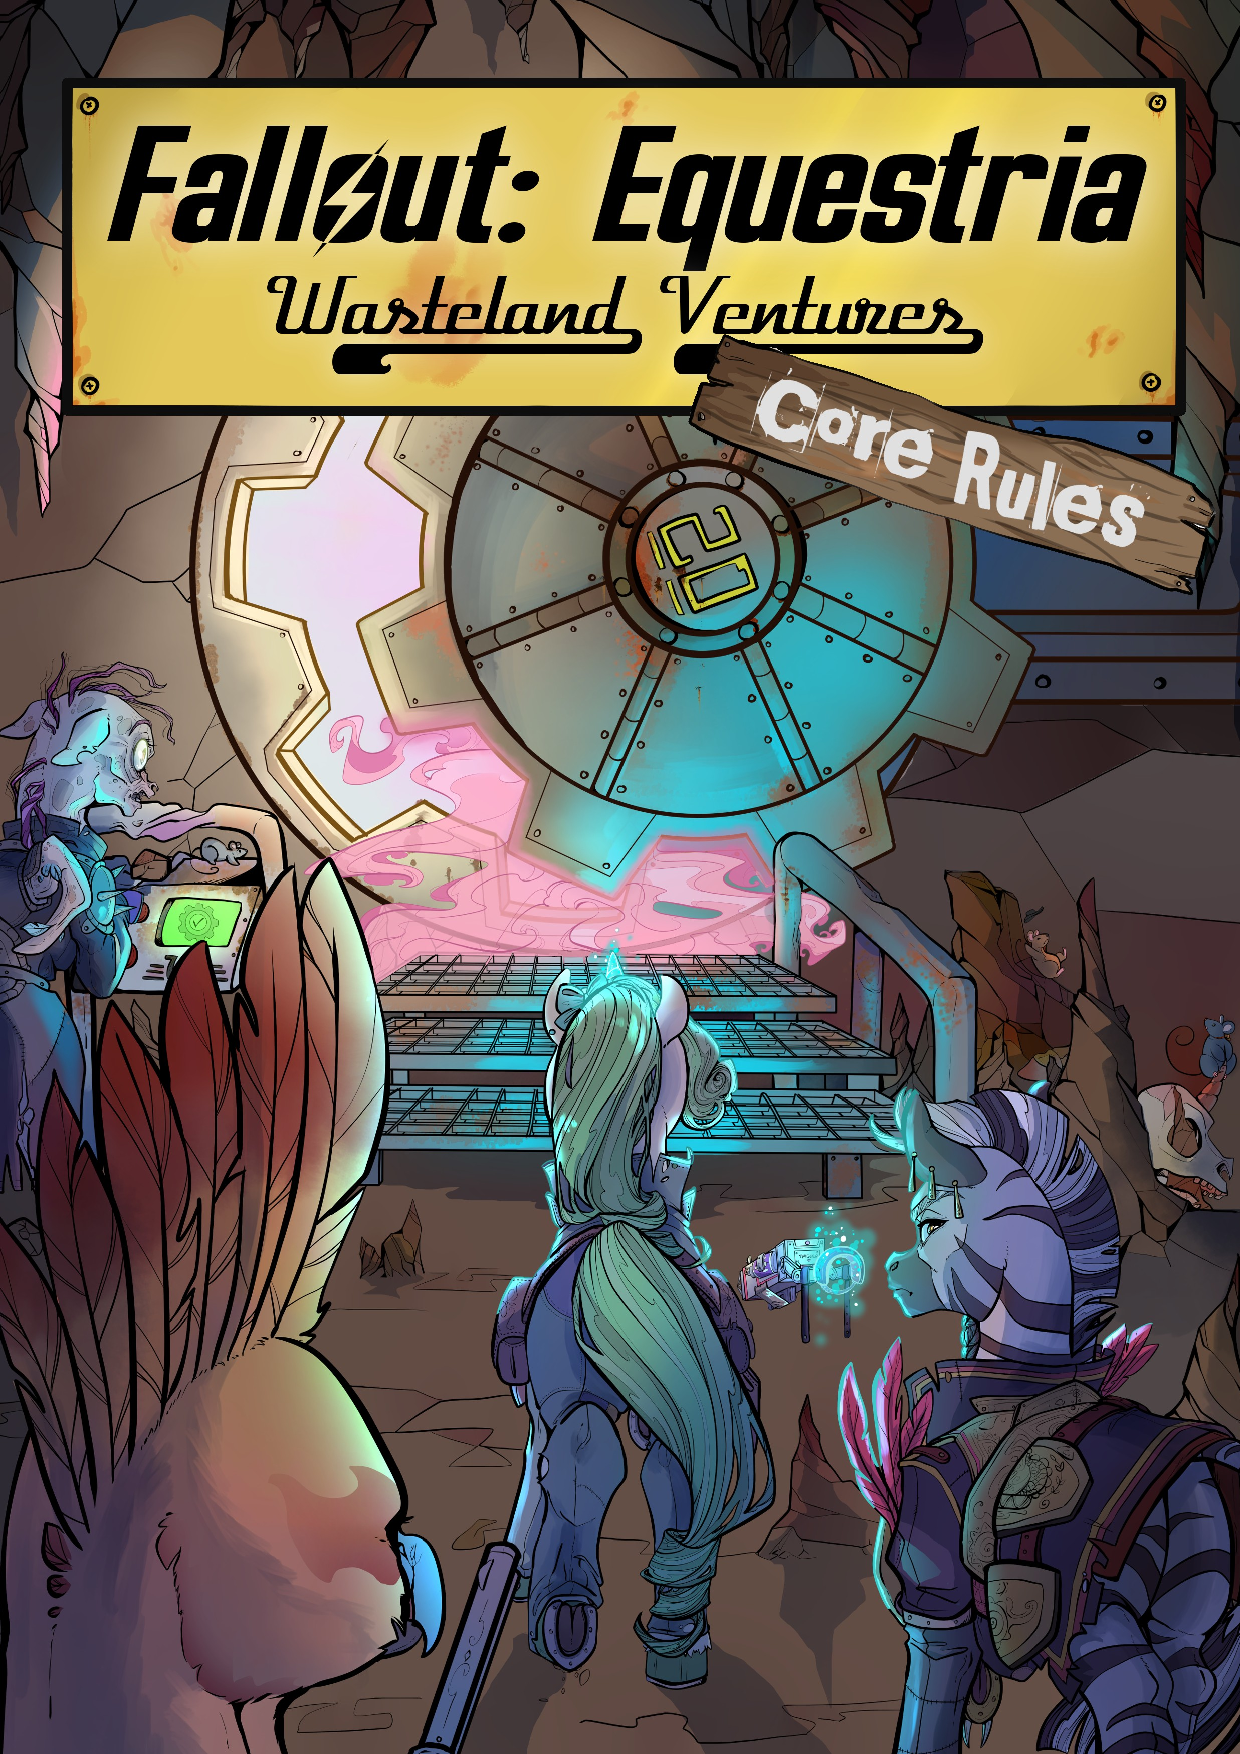
\includepdf[pages={1}]{WORD/COVER-CORE.pdf}	
	\onecolumn	
	\setcounter{page}{1}
	\begin{center}
		Compiled by Waak, Kireanikin, LaPa, Miksu \& SourCherry
		
		10 AP rule basis by Yondalor
		
		Token HP \& Status rule bases by LZ
		
		\bigskip		
		\textbf{Playtesting and Advice:} LZ, Moonlight, Mittens, Kittyfluff, Ray\_Lionheart, f1r3w4rr10r, Tierney Kelly, Eden, Kendallkun, Pesian, Raven, dumbhat, GODOG, Borealis
		
		\bigskip
		\textbf{Cover and Graphics:} SourCherry
		
		\bigskip
		\textbf{Layout:} Waak
	\end{center}
	
	\vfill
	
	\begin{center}
		\textbf{Version 1.4}
		
		\emph{Last compiled on \thedate}
        
        \emph{\textbf{Contact:} wasteland-ventures@googlegroups.com}
	\end{center}	

	\begin{figure*}[bp]
		\centering
		
\includegraphics[width=3cm]{Art/ISA_Logo}
		\label{fig:isalogo}
	\end{figure*}

	\tableofcontents
	
	\chapter{Introduction}
	\noindent
	Within this document is listed the items of any kind within \emph{Fallout Equestria: Wasteland Ventures} rules. Be they valuables or junk, crafting parts of complete items, they can be found within these pages.
	
	Below is a quick list of phrases that frequently appear in the statistics of items, each having a quick description added to them.
	
	\chapter{Weapons}
	\noindent
	Lets be frank, in the Wasteland one doesn't survive long without a trustworthy weapon on their side. True, one can utilize their natural physique to down their opponents, or avoid combat entirely, but a little extra never hurts - one can call it ''insurance''.	
	
	You have a few categories to choose your weapon from, listed in the following order:
	
	\begin{verse}
		\textbf{Firearms} - the conventional method of dispatching an enemy from afar. Engineered simultaneously by Earth ponies, Griffins, and Zebras, a wide range of possibilities exist from small pistols to heavy machine guns.
		
		\textbf{Magical Energy Weapons} - the more advanced weapons engineered by both Unicorns and Zebras, these guns, shortened as MEW, utilize arcane or spiritual energies to draw devastating power onto the field.
		
		\textbf{Explosives} - for things that go boom.
		
		\textbf{Melee} - the more honorable way of handling things, close and personal.
		
		\textbf{Unarmed} - you cannot be stripped of weapons, because you are a weapon.
	\end{verse}
	
	Under each weapon is listed a list of \textbf{Modifications} you can apply to the weapon, and change the characteristics more to your liking. Provided you have the caps, you can potentially prolong the time you use a specific weapon through modifying and upgrading it.
	
	Below is a quick list of phrases that frequently appear in the statistics of weapons, each having a quick description added to them.
	
	\clearpage
	{
		\rowcolors{1}{gray!30}{gray!10}
		\begin{tabu} to 150mm{| X[l,1] | X[l,3] |}
			\hline
			\cellcolor{gray!50} Name & \cellcolor{gray!50}Description                                                                            \\ \hline
			Holdout Weapon           & The weapon is small enough to be hidden amidst clothing or items.                                         \\
			Damage                   & The amount of damage the weapon deals per hit. Number in parenthesis represents the number of dice thrown \\
			DT Reduction             & How much DT the Magical Energy Weapon ignores when it hits a target.                                      \\
			Firing Mode              & Tells how the ranged weapon operates. The different modes are as follows:                                 \\
			Single Shot (SS)         & After each shot, ammo must be reloaded with Reload action                                                 \\
			Bolt Action (BA)         & After each shot, manual chambering. Thus slower rate of fire                                              \\
			Semi-Auto (SA)           & The weapon chambers a new round to be fired with the next pull of the trigger, faster than Bolt Action    \\
			Full Auto (5F-20F)       & For each 5 rounds fired, a roll is made. Cumulative -10 penalty to rolls after the first.                 \\
			Action Points (AP)       & The cost of attacking with the weapon in AP                                                               \\
			Ammo                     & The ammo the ranged weapon uses.                                                                          \\
			Capacity                 & The maximum amount of ammo the ranged weapon can hold                                                     \\
			Reload Type              & Lists how the weapon is reloaded. The different types are as follows:                                     \\
			Clip (C)                 & A clip or detachable magazine. Reload fills the entire Capacity                                           \\
			Cylinder (CY)            & A non-detachable chamber and ammo magazine. Reload fills the entire Capacity                              \\
			Battery (B)              & Magic-powered. Reload fills the entire Capacity.                                                          \\
			Internal (I)             & Internal magazine. One Reload action loads one Ammo                                                       \\
			Reload AP                & The AP cost of Reload action with the weapon                                                              \\
			Range                    & The effective ranges of the weapon in meters: Short / Medium / Long                             \\
			Blast Radius             & Tells the area of effect of the explosive, using Burst Templates                                          \\
			Weight                   & The weight of the weapon in kilograms                                                                     \\
			STR req.                 & How much Strength the character must have to utilize the weapon without penalties                         \\
			Value                    & The value of the weapon in bottlecaps                                                                     \\
			Type                     & The weapon's category. Perks refer to this when providing bonuses to specific weapon categories           \\
			Special Attack           & A non-standard attack one can use with the melee or unarmed weapon.                                       \\
			Notes                    & Further notes, special rules and the like                                                                 \\ \hline
		\end{tabu} 
	}
	
	\clearpage
	\section*{Firearms}
	\addcontentsline{toc}{section}{Firearms}
	
	\subsection*{Pistols}
	\addcontentsline{toc}{section}{Pistols}
	
	{
		\rowcolors{1}{gray!30}{gray!10}		
		Buckington ``Peashooter''
		
		\begin{tabu} to 150mm{| X[c,2] | X[c,2] | X[c,1] | X[c,2] | X[c,1] | X[c,2] | X[c,2] | X[c,3] | X[c,1] | X[c,1] | X[c,1] | X[c,1] |}
			\hline
			DMG & Firing Mode & AP & Ammo & Cap. & Reload Type & Reload AP & Range & Wgt & STR req. & Value & Type \\
			(1) &	SA &	3	& .22LR  &	16 &	C	 &4 &	10/20/40 &	1 kg &	1 &	20 &	Pistol 
		\end{tabu}
	}
	Completely Silent: no penalty on Sneak after Sneak Attack.
	
	\bigskip
	
	Damage	Firing Mode	AP	Ammo	Capacity	Reload Type	Reload AP	Range (meters)			Weight	STR req.	Value	Type	Notes
	Holdout Weapon								S	M	L					

	+ Ext. Mag	-	-	-	-	25	-	5	-	-	-	+ 0,1 kg	-	30	Mod	
	+ Pocket Frame	-	-	-	-	-	-	-	8	16	32	- 0,3 kg	-	50	Mod	Can be placed in a Quick Slot
	
	
	
	
\end{document}